\chapter{Additional content}

\clearpage
\section{\acs{emel} paper forms}
\begin{figure}[htbp]
  \caption{Front page of the paper form used by \acs{emel} during vehicle maintenance. Operators use this section to record identified malfunctions.}
  \centering
  \includegraphics[width=0.50\textwidth]{figs/chapter2/emel_front}
  \label{fig:emel_front}
\end{figure}

\begin{figure}[htbp]
  \caption{Back page of the paper form used by \acs{emel} during vehicle maintenance. Mechanics use this section to document the parts replaced during the repair process.}
  \centering
  \includegraphics[width=0.50\textwidth]{figs/chapter2/emel_back}
  \label{fig:emel_back}
\end{figure}

\clearpage
\section{\ac{servqual}}
\subsection{\ac{servqual} in CMV SA dealership}

\begin{figure}[htbp]
  \caption{\ac{servqual} statements used by the authors in the study to measure the quality of the service at a CMV SA dealership in South Africa (~\cite{Measuring_After_sales_Service_Quality}).}
  \centering
  \includegraphics[width=0.75\textwidth]{figs/SERVQUAL_statements}
  \label{fig:SERVQUAL_statements}
\end{figure}


\begin{figure}[htbp]
  \caption{\ac{servqual} results of the study to measure the quality of the service at a CMV SA dealership in South Africa. In the table the header "Exp" means the expectation, "Per" means the perception, "Zc" means the Service quality score from the customers and the "Zc-ms" means Service quality score measure by the difference of the expectations of the customer and the expectation of the dealers. (~\cite{Measuring_After_sales_Service_Quality})}
  \centering
  \includegraphics[width=0.75\textwidth]{figs/SERVQUAL_results}
  \label{fig:SERVQUAL_results}
\end{figure}

\clearpage
\subsection{\ac{servqual} questionaire}

\begin{table}[ht]
\centering
\resizebox{0.75\textwidth}{!}{%
\begin{tabular}{p{2.5cm} p{6cm} p{6cm} p{1.5cm}}
\hline
\textbf{Dimension} & \textbf{Expectation Survey} & \textbf{Perception Survey} & \textbf{Gap} \\
\hline 
Tangibility & E1. Excellent companies will have modern-looking equipment. & P1. XYZ company has modern-looking equipment. & E - P \\
 & E2. The physical facilities at excellent companies will be visually appealing. & P2. XYZ company’s physical facilities are visually appealing. & \\
 & E3. Employees of excellent companies will be neat-appearing. & P3. XYZ company’s employees are neat-appearing. & \\
 & E4. Materials associated with the service (such as pamphlets or statements) will be visually appealing in excellent companies. & P4. Materials associated with the service (such as pamphlets or statements) are visually appealing at XYZ company. & \\
\hline
Reliability & E5. When excellent companies promise to do something by a certain time, they do so. & P5. When XYZ company promises to do something by a certain time, it does so. & \\
 & E6. When customers have a problem, excellent companies will show sincere interest in solving it. & P6. When you have a problem, XYZ company shows a sincere interest in solving it. & \\
 & E7. Excellent companies will perform the service right the first time. & P7. XYZ company performs the service right the first time. & \\
 & E8. Excellent companies will provide the services at the time they promise to do so. & P8. XYZ company provides its services at the time it promises to do so. & \\
 & E9. Excellent companies will insist on error-free records. & P9. XYZ company insists on error-free records. & \\
\hline
Responsiveness & E10. Employees of excellent companies will tell customers exactly when services will be performed. & P10. Employees of XYZ company tell you exactly when services will be performed. & \\
 & E11. Employees of excellent companies will provide prompt services to customers. & P11. Employees of XYZ company give you prompt service. & \\
 & E12. Employees of excellent companies will always be willing to help customers. & P12. Employees of XYZ company are always willing to help you. & \\
 & E13. Employees of excellent companies will never be too busy to respond to customers. & P13. Employees of XYZ company are never too busy to respond to your requests. & \\
\hline
Assurance & E14. The behavior of employees at excellent companies will instill confidence in customers. & P14. The behavior of employees of XYZ company instills confidence in customers. & \\
 & E15. Customers of excellent companies will feel safe in their transactions. & P15. You feel safe in your transactions with XYZ company. & \\
 & E16. Employees of excellent companies will be consistently courteous with customers. & P16. Employees of XYZ company are consistently courteous with you. & \\
 & E17. Employees of excellent companies will have the knowledge to answer customers’ questions. & P17. Employees of XYZ company have the knowledge to answer your questions. & \\
\hline
Empathy & E18. Excellent companies will give customers individual attention. & P18. XYZ company gives you individual attention. & \\
 & E19. Excellent companies will have operating hours convenient to all their customers. & P19. XYZ company has operating hours convenient to all its customers. & \\
 & E20. Excellent companies will have employees who give customers personal attention. & P20. XYZ company has employees who give you personal attention. & \\
 & E21. Excellent companies will have customer’s best interests at heart. & P21. XYZ company has your best interests at heart. & \\
 & E22. The employees of excellent companies will understand the specific needs of their customers. & P22. Employees of XYZ company understand your specific needs. & \\
\hline
\end{tabular}
}
\caption{\ac{servqual} Questionnaire Template (Expectations vs Perceptions) ~\cite{master_servqual_model}} 
\label{table:servqual_template}
\end{table}

\clearpage
\section{Maintenance flow chart}


\begin{figure}[h]
  \caption{Use case flow chart of dealership maintenance, with statuses grouped by use cases}
  \centering
  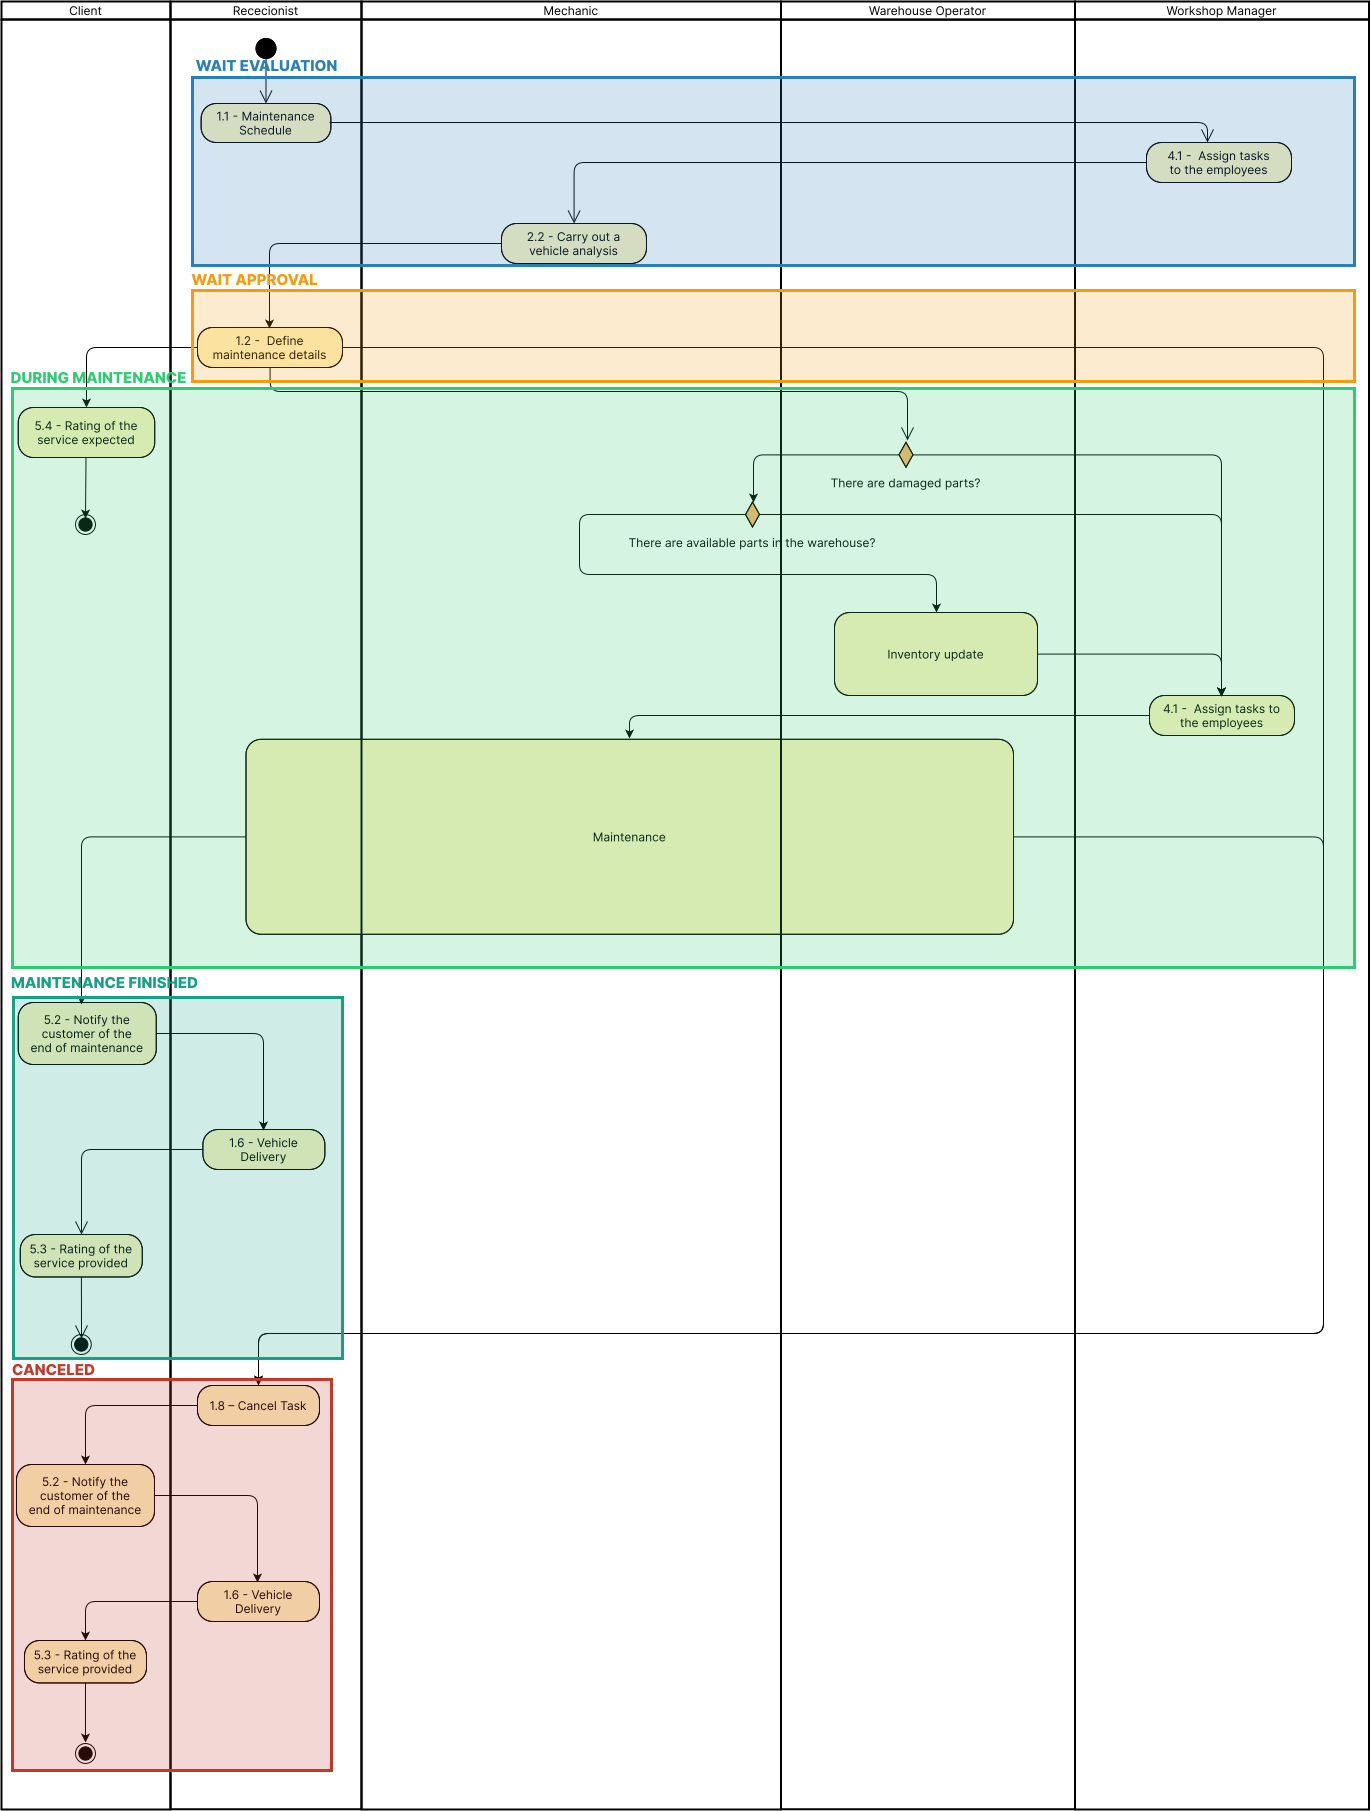
\includegraphics[width=0.90\textwidth]{figs/Status/Maintenance/UseCaseStatus}
  \label{fig:maintenanceUseCaseStatus}
\end{figure}


\begin{figure}[h]
  \caption{Use case flow chart of an entity managing maintenance without evaluation, with statuses grouped by use cases}
  \centering
  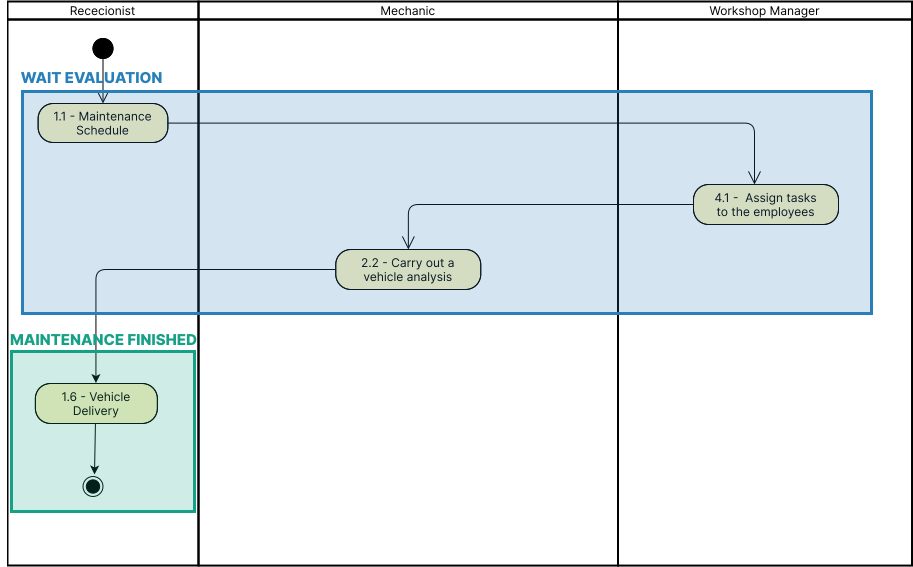
\includegraphics[width=\textwidth]{figs/Status/Maintenance/EntityDiagram}
  \label{fig:maintenanceDealershipUseCaseStatus}
\end{figure}

\section{Database indexes}


\foreach \p in {1,...,4}{%  <-- change 5 to the total number of pages
\begin{figure}[p]
  \caption{Database indexes— page \p}
  \centering
  \includegraphics[page=\p,width=\textwidth]{figs/dbDiagrams/BD_indexes}
  \label{fig:BD_indexes-\p}
\end{figure}
}

\clearpage
\section{Application implementation images}

\subsection{Rececionist}


\subsubsection{Create Client}


\begin{figure}[htbp]
  \caption{Example of the confirmation email sent to the client. The layout used for dealership employees is similar.}
  \centering
  \includegraphics[width=0.80\textwidth]{figs/Implementation/rececionist/CreateClient}
  \label{fig:CreateClient}
\end{figure}


\begin{figure}[htbp]
  \caption{Form where the client fills in the remaining required personal information.}
  \centering
  \includegraphics[width=0.80\textwidth]{figs/Implementation/rececionist/SetPassword}
  \label{fig:SetPassword}
\end{figure}

\clearpage
\subsubsection{Active Maintenance}

\begin{figure}[htbp]
  \caption{Active maintenance details Information tab.}
  \centering
  \includegraphics[width=\textwidth]{figs/Implementation/rececionist/maintenance_details}
  \label{fig:impReceMaintHome}
\end{figure}

\begin{figure}[htbp]
  \caption{Active maintenance details task tab.}
  \centering
  \includegraphics[width=\textwidth]{figs/Implementation/rececionist/maintenance_details_task}
  \label{fig:impReceMaintTask}
\end{figure}

\begin{figure}[htbp]
  \caption{Active maintenance details change tab.}
  \centering
  \includegraphics[width=\textwidth]{figs/Implementation/rececionist/maintenance_details_change}
  \label{fig:impReceMaintChange}
\end{figure}



\clearpage
\subsection{Mechanic}

\subsubsection{Maintenance Normal Task}

\begin{figure}[htbp]
  \caption{Mechanic completing simple task first step.}
  \centering
  \includegraphics[width=\textwidth]{figs/Implementation/mechanic/MechanicTaskNormal}
  \label{fig:MechanicTaskNormal}
\end{figure}



\begin{figure}[htbp]
  \caption{Change task modal.}
  \centering
  \includegraphics[width=\textwidth]{figs/Implementation/mechanic/MechanicTaskChangeTask}
  \label{fig:MechanicTaskChangeTask}
\end{figure}


\begin{figure}[htbp]
  \caption{Mechanic task last step.}
  \centering
  \includegraphics[width=\textwidth]{figs/Implementation/mechanic/MechanicTaskLastStep}
  \label{fig:MechanicTaskLastStep}
\end{figure}


\subsubsection{Vehicle Evaluation}


\begin{figure}[htbp]
  \caption{Mechanic select part modal.}
  \centering
  \includegraphics[width=\textwidth]{figs/Implementation/mechanic/MechanicEvaluationSelectTaskWitPart}
  \label{fig:MechanicEvaluationSelectTaskWitPart}
\end{figure}

\begin{figure}[htbp]
  \caption{Mechanic Evaluation task with part selected.}
  \centering
  \includegraphics[width=\textwidth]{figs/Implementation/mechanic/TaskSelected}
  \label{fig:TaskSelected}
\end{figure}



\begin{figure}[htbp]
  \caption{Mechanic Evaluation last step.}
  \centering
  \includegraphics[width=\textwidth]{figs/Implementation/mechanic/EvaluationLastStep}
  \label{fig:EvaluationLastStep}
\end{figure}


\clearpage
\subsection{Warehouse Manager}

\subsubsection{Inventory}

\begin{figure}[htbp]
  \caption{Inventory editor.}
  \centering
  \includegraphics[width=\textwidth]{figs/Implementation/warehouse/inventoryEdit}
  \label{fig:inventoryEdit}
\end{figure}

\subsubsection{Purchases}


\begin{figure}[htbp]
  \caption{Assgined purchase details.}
  \centering
  \includegraphics[width=\textwidth]{figs/Implementation/warehouse/PurchaseDetails}
  \label{fig:PurchaseDetails}
\end{figure}


\begin{figure}[htbp]
  \caption{Waiting delivery purchase details.}
  \centering
  \includegraphics[width=\textwidth]{figs/Implementation/warehouse/PurchaseRegisterParts}
  \label{fig:PurchaseRegisterParts}
\end{figure}


\begin{figure}[htbp]
  \caption{Delivered purchase details.}
  \centering
  \includegraphics[width=\textwidth]{figs/Implementation/warehouse/PurchaseFinishedDetails}
  \label{fig:PurchaseFinishedDetails}
\end{figure}

\subsubsection{Supplier}


\begin{figure}[htbp]
  \caption{Supplier details.}
  \centering
  \includegraphics[width=\textwidth]{figs/Implementation/warehouse/supplierDetails}
  \label{fig:supplierDetails}
\end{figure}


\clearpage
\subsection{Workshop Manager}

\subsubsection{Assign Task}

\begin{figure}[htbp]
  \caption{Assign task to a mechanic.}
  \centering
  \includegraphics[width=\textwidth]{figs/Implementation/workshopmanager/addTask}
  \label{fig:workshopmanagerAssignTask}
\end{figure}

\subsubsection{Maintenance}

\begin{figure}[htbp]
  \caption{Active maintenance list.}
  \centering
  \includegraphics[width=\textwidth]{figs/Implementation/workshopmanager/maintenanceList}
  \label{fig:workshopmanagerMaintenanceList}
\end{figure}


\begin{figure}[htbp]
  \caption{Maintenance details information tab.}
  \centering
  \includegraphics[width=\textwidth]{figs/Implementation/workshopmanager/maintenanceDetails}
  \label{fig:workshopmanagerMaintenanceDetails}
\end{figure}

\begin{figure}[htbp]
  \caption{Maintenance details tasks tab.}
  \centering
  \includegraphics[width=\textwidth]{figs/Implementation/workshopmanager/maintenanceDetailsTask}
  \label{fig:workshopmanagerMaintenanceDetailsTask}
\end{figure}


\begin{figure}[htbp]
  \caption{Report example.}
  \centering
  \includegraphics[width=\textwidth]{figs/Implementation/workshopmanager/report}
  \label{fig:report}
\end{figure}

\subsubsection{Purchase}

\begin{figure}[htbp]
  \caption{Purchase request details.}
  \centering
  \includegraphics[width=\textwidth]{figs/Implementation/workshopmanager/purchaseDetails}
  \label{fig:workshopmanagerPurchaseDetails}
\end{figure}

\subsubsection{Supplier}

\begin{figure}[htbp]
  \caption{Supplier list.}
  \centering
  \includegraphics[width=\textwidth]{figs/Implementation/workshopmanager/supplierList}
  \label{fig:workshopmanagerSupplierList}
\end{figure}

\begin{figure}[htbp]
  \caption{Supplier Details.}
  \centering
  \includegraphics[width=\textwidth]{figs/Implementation/workshopmanager/supplierDetails}
  \label{fig:workshopmanagerupplierDetails}
\end{figure}

\subsubsection{Workers}

\begin{figure}[htbp]
  \caption{Worker details.}
  \centering
  \includegraphics[width=\textwidth]{figs/Implementation/workshopmanager/workerDetails}
  \label{fig:workerDetails}
\end{figure}



\begin{figure}[htbp]
  \caption{Create worker.}
  \centering
  \includegraphics[width=\textwidth]{figs/Implementation/workshopmanager/workerCreate}
  \label{fig:workerCreate}
\end{figure}

\clearpage
\subsection{Client}

\subsubsection{Email Notification}


\begin{figure}[htbp]
  \caption{Client email notification of the end of the maintenance.}
  \centering
  \includegraphics[width=\textwidth]{figs/Implementation/client/MaintenanceFinishedNotification}
  \label{fig:MaintenanceFinishedNotification}
\end{figure}

\subsubsection{Application layout}

\begin{figure}[htbp]
  \caption{Client home page with no active maintenance.}
  \centering
  \includegraphics[width=0.30\textwidth]{figs/Implementation/client/MaintenanceNoState}
  \label{fig:MaintenanceNoState}
\end{figure}



\begin{figure}[htbp]
  \caption{Client Home page when he schedules a maintenance with the rececionist.}
  \centering
  \includegraphics[width=0.30\textwidth]{figs/Implementation/client/MaintenanceState1}
  \label{fig:MaintenanceState1}
\end{figure}




\begin{figure}[htbp]
  \caption{Client Home page when the maintenance is approved.}
  \centering
  \includegraphics[width=0.30\textwidth]{figs/Implementation/client/MaintenanceState3}
  \label{fig:MaintenanceState3}
\end{figure}


\begin{figure}[htbp]
  \caption{Client Home page when the maintenance tasks are completed and the client can go take the vehicle.}
  \centering
  \includegraphics[width=0.30\textwidth]{figs/Implementation/client/MaintenanceState4}
  \label{fig:MaintenanceState4}
\end{figure}

\subsubsection{Client Questionaires}

\begin{figure}[htbp]
  \caption{Client Expectation Questionaire refering the questions and introduction in ~\cite{master_servqual_model}.}
  \centering
  \includegraphics[width=0.30\textwidth]{figs/Implementation/client/ExpectationQuestionare}
  \label{fig:ExpectationQuestionare}
\end{figure}


\begin{figure}[htbp]
  \caption{Client Perception Questionaire refering the questions and introduction in ~\cite{master_servqual_model}.}
  \centering
  \includegraphics[width=0.30\textwidth]{figs/Implementation/client/PerceptionQuestionare}
  \label{fig:PerceptionQuestionare}
\end{figure}

\subsubsection{Maintenance History}

\begin{figure}[htbp]
  \caption{Details of a maintenance example the tab of information.}
  \centering
  \includegraphics[width=0.25\textwidth]{figs/Implementation/client/MaintenanceDetailsInfo}
  \label{fig:MaintenanceDetailsInfo}
\end{figure}


\begin{figure}[htbp]
  \caption{Details of a maintenance example the list of task.}
  \centering
  \includegraphics[width=0.25\textwidth]{figs/Implementation/client/MaintenanceDetailsTasks}
  \label{fig:MaintenanceDetailsTasks}
\end{figure}

\clearpage
\subsection{Dealership Admin}


\subsubsection{Manage Parts}

\begin{figure}[htbp]
  \caption{Parts type details.}
  \centering
  \includegraphics[width=\textwidth]{figs/Implementation/dealershipAdmin/partsDetails}
  \label{fig:partsDetails}
\end{figure}

\begin{figure}[htbp]
  \caption{Parts type edit.}
  \centering
  \includegraphics[width=\textwidth]{figs/Implementation/dealershipAdmin/partsEdit}
  \label{fig:partsEdit}
\end{figure}

\begin{figure}[htbp]
  \caption{Parts type delete.}
  \centering
  \includegraphics[width=\textwidth]{figs/Implementation/dealershipAdmin/partsDelete}
  \label{fig:partsDelete}
\end{figure}


\begin{figure}[htbp]
  \caption{Parts type create.}
  \centering
  \includegraphics[width=\textwidth]{figs/Implementation/dealershipAdmin/partsCreate}
  \label{fig:partsCreate}
\end{figure}


\clearpage
\subsubsection{Manage Normal Tasks}

\begin{figure}[htbp]
  \caption{Task type list index.}
  \centering
  \includegraphics[width=\textwidth]{figs/Implementation/dealershipAdmin/taskIndex}
  \label{fig:taskIndex}
\end{figure}

\begin{figure}[htbp]
  \caption{Task type edit.}
  \centering
  \includegraphics[width=\textwidth]{figs/Implementation/dealershipAdmin/taskEdit}
  \label{fig:taskEdit}
\end{figure}


\begin{figure}[htbp]
  \caption{Task type details.}
  \centering
  \includegraphics[width=\textwidth]{figs/Implementation/dealershipAdmin/taskDetails}
  \label{fig:taskDetails}
\end{figure}

 
\begin{figure}[htbp]
  \caption{Task type delete.}
  \centering
  \includegraphics[width=\textwidth]{figs/Implementation/dealershipAdmin/taskDelete}
  \label{fig:taskDelete}
\end{figure}

\begin{figure}[htbp]
  \caption{Task type create.}
  \centering
  \includegraphics[width=\textwidth]{figs/Implementation/dealershipAdmin/taskCreate}
  \label{fig:taskCreate}
\end{figure}


\subsubsection{Manage Evaluation Tasks}


\begin{figure}[htbp]
  \caption{Eval task list index.}
  \centering
  \includegraphics[width=\textwidth]{figs/Implementation/dealershipAdmin/evalIndex}
  \label{fig:evalIndex}
\end{figure}
 
\begin{figure}[htbp] 
  \caption{Eval task edit.}
  \centering
  \includegraphics[width=\textwidth]{figs/Implementation/dealershipAdmin/evalEdit}
  \label{fig:evalEdit} 
\end{figure}




\begin{figure}[htbp]
  \caption{Eval task create.}
  \centering
  \includegraphics[width=\textwidth]{figs/Implementation/dealershipAdmin/evalCreate}
  \label{fig:evalCreate}
\end{figure}

\begin{figure}[htbp]
  \caption{Eval task delete.}
  \centering
  \includegraphics[width=\textwidth]{figs/Implementation/dealershipAdmin/evalDelete}
  \label{fig:evalDelete}
\end{figure}

\begin{figure}[htbp]
  \caption{Eval task details.}
  \centering
  \includegraphics[width=\textwidth]{figs/Implementation/dealershipAdmin/evalDetails}
  \label{fig:evalDetails}
\end{figure}

\section{Usability test tasks}

\foreach \p in {1,...,11}{%  <-- change 5 to the total number of pages
\begin{figure}[p]
  \caption{User tests tasks — page \p}
  \centering
  \includegraphics[page=\p,width=\textwidth]{figs/chapter5/UserTestsTasksEnglish}
  \label{fig:UserTestsTasks-\p}
\end{figure}
}

\section{Usability test questionaire}

\foreach \p in {1,...,6}{%  <-- change 5 to the total number of pages
\begin{figure}[p]
  \caption{Aplication questionaire— page \p}
  \centering
  \includegraphics[page=\p,width=\textwidth]{figs/chapter5/AplicationQuestionaire}
  \label{fig:AplicationQuestionaire-\p}
\end{figure}  
}




